% !TEX root = bleb.tex


%%%%%%%%%%%%%%%%%%%%%%%%%%%%%%%%%%%%%%%%%%%%%%%%%%%
\section{Results}
%%%%%%%%%%%%%%%%%%%%%%%%%%%%%%%%%%%%%%%%%%%%%%%%%%%


%%%%%%%%%%%%%%%%%%%%%%%%%%%%%%%%%%%%%%%%%%%%%%%%%%%
\subsection{Model exhibits  blebbing and non-blebbing behaviors.}
%%%%%%%%%%%%%%%%%%%%%%%%%%%%%%%%%%%%%%%%%%%%%%%%%%%
The quantitative model combines five mechanisms of the membrane-cortex interaction: force-sensitive adhesions, local hydrostatic pressure, cortex contractility, membrane tension and cortex turnover. We numerically simulate the model and find three classes of dynamics arise from the same model at different parameters: Stable non-blebbing states, stationary blebbing, and traveling blebs. We discuss these in turn.

% stationary blebs
At equilibrium, the membrane and cortex are locally approximately flat. We apply an initial perturbation corresponding to local ablation by locally reducing the adhesion density by 99\%. In blebbing states, the membrane will detach from the cortex and protrude locally. The membrane  then continues to move away from the thinning cortex as the detached region grows in both lateral size (along the surface) and in height (i.e., normal to the cell surface) until it reaches a maximum size around $\tau=1.75$. The adhesions subsequently accumulate under the protruding membrane and the cortex is able to re-attach and thicken. Under the influence of cortex contraction, the bleb heals and the membrane returns to its equilibrium. This bleb-like behavior is observed in 2D (Fig.~\ref{fig::stationary}A left) and in 3D (Fig.~\ref{fig::stationary}B) simulations. 
% stable
In contrast, at different biophysical parameters, the detached region of membrane may not grow after perturbation, but instead directly and rapidly return to equilibrium, shown in Fig.~\ref{fig::stationary}A right. This stable behavior is observed in both 2D (Fig.~\ref{fig::stationary}A right) and in 3D (not shown). 

%%%%%%%%%%%%%%%%%%%%%%%%%%%%%%%%%%%%%%%%%%%%%%%%%%%%%%%%%%%%%%%%%%%%%%%%
\begin{figure}
\captionsetup{width=17cm}
	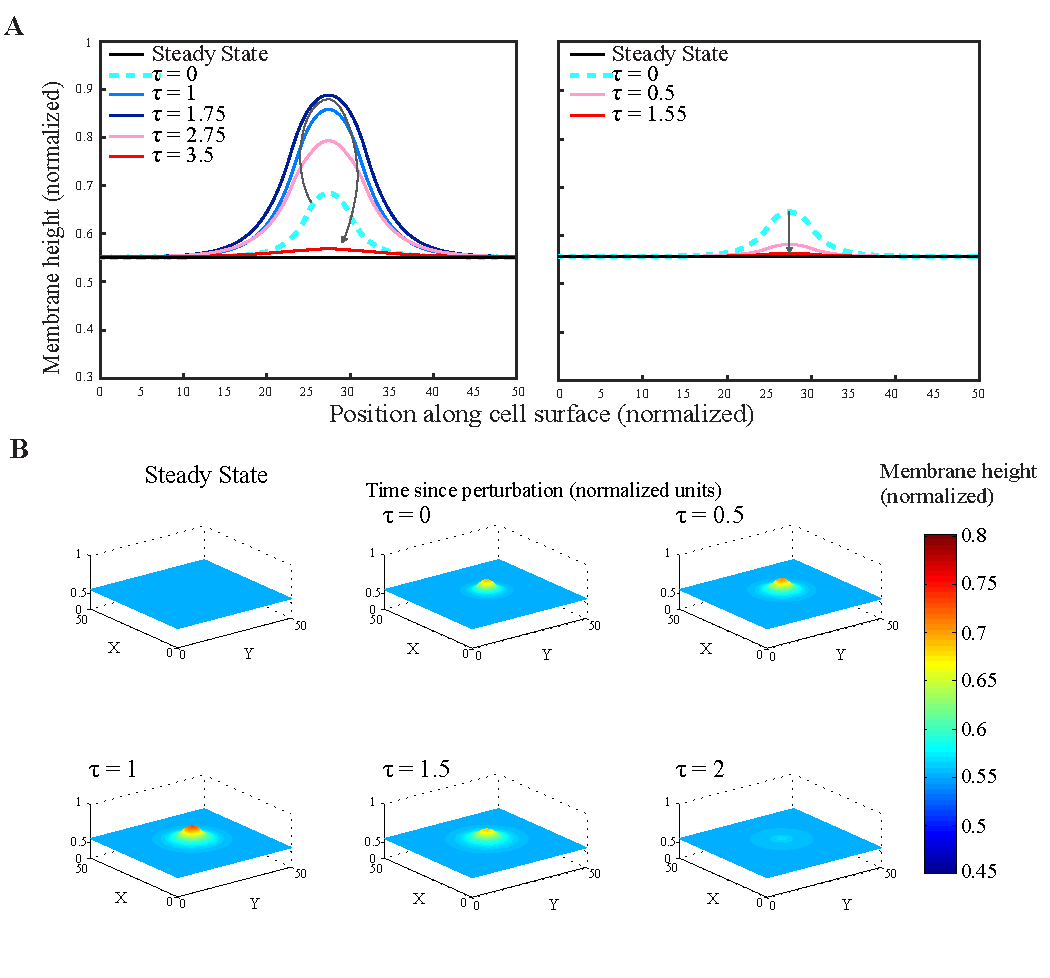
\includegraphics[width=17cm,center]{Project1/figs/figure2}
      \caption{Model exhibits stationary blebs and non-blebbing states in 2D and 3D. (A) Profile of stationary solution of the 2D system: (Left) Excitable state in which an initial perturbation (cyan dashed) expands in both height (normal to cell surface) and laterally along cell surface before retracting. (Right) Non-excitable state in which the initial perturbation rapidly and directly returns to equilibrium. Parameter values: $\Omega = 40$, $\epsilon = 0.1$, $F_0 = 1$, $M = 0.007$, $P = 0.1$ and $D = 0.15$ for the excitable state, $D = 0.2$ for the non-excitable state. (B) Profile of stationary solution  of the 3D system in an excitable state. Parameter values: $\Omega = 50$, $\epsilon = 0.1$, $F_0 = 1$, $M = 0.007$, $P = 0.1$ and $D = 0.15$. Note that our choice of nondimensionalization means that only relative changes in $Y_M$ and $Y_C$ are physically meaningful.}
      \label{fig::stationary}
\end{figure}
%%%%%%%%%%%%%%%%%%%%%%%%%%%%%%%%%%%%%%%%%%%%%%%%%%%%%%%%%%%%%%%%%%%%%%%%


%Interestingly, the model can also exhibit another bleb-like behavior. In this third scenario, the membrane will continue to move away from the thinning cortex and grow in size and manages to trigger a travelling wave of membrane detachment followed by a travelling wave of cortex contraction. This travelling bleb behavior is observed in 2D (Figure 4A) and in 3D (Figure 4B).



%%%%%%%%%%%%%%%%%%%%%%%%%%%%%%%%%%%%%%%%%%%%%%%%%%%
\subsection{Blebs as excitable phenomena}
%%%%%%%%%%%%%%%%%%%%%%%%%%%%%%%%%%%%%%%%%%%%%%%%%%%

% simplification to ODEsys
While numerical simulation of the full model reveals a range of blebbing behavior, we seek to elucidate how biophysical parameters determine the class of dynamics, specifically whether or not a bleb forms. To this end, we simplify the model by neglecting the tension term in Eq.~\ref{eq::nondimyM}. Heuristically, we model an (unrealistic) system in which a patch of cell surface has been cut off from its neighbors (as in Fig. \ref{fig::blebgeometry}). This transforms the force-balance equations Eq.~\ref{eq::nondimyM}-\ref{eq::nondimyC} into a pair of algebraic equations,
\begin{align}
Y_M &= \frac{(A+CM)P}{A MC + AP + MCP}\label{eq::ODEyM}\\
Y_C &= \frac{AP}{A MC + AP + MCP}\label{eq::ODEyC},
\end{align}
shown in Fig.~\ref{fig::ODE}A as a function of $A$ and $C$. These are then substituted into the assembly/disassembly equations, yielding
\begin{align}
\frac{d C}{d \tau} &= \Omega A - C \label{eq::ODEC}\\
\epsilon \frac{d A}{d \tau} &= \frac{C}{1+C} \mbox{exp}\left( -\frac{1}{D} \frac{MP C}{A MC + AP + MCP}\right) \notag\\
 &- A\; \mbox{exp}\left( + \frac{1}{F_0}\frac{MP C}{A MC + AP + MCP}\right) \label{eq::ODEA}
\end{align}
The model is now a system of two ordinary differential equations (ODEs) amenable to phase plane analysis \cite{Keshet}. We plot nullclines in which $dA/d\tau=0$ (green) or $dC/d\tau=0$ (orange) in Fig.~\ref{fig::ODE}B,D.
% nullcline analysis
Four regimes of behavior are observed in this system: 
% monostable
In one (top-left), there is a single stable equilibrium with no threshold behavior. In this regime, perturbations rapidly return to their steady state. We identify this with the stable non-blebbing behavior of the full model. 

%%%%%%%%%%%%%%%%%%%%%%%%%%%%%%%%%%%%%%%%%%%%%%%%%%%%%%%%%%%%%%%%%%%%%%%%
\begin{figure}
   \begin{center}
   \captionsetup{width=17cm}
     \includegraphics*[width=17cm,center]{Project1/figs/figure3}
      \caption{Emergence of blebbing states can be understood in terms of the local $A-C$ phase plane. (A) Since the model assumed force-balance between adhesions, cortex and membrane, a particular value of $A$ and $C$ determine the current position of the membrane and cortex $y_M$ and $y_C$ via Eq.~\ref{eq::ODEyM}-\ref{eq::ODEyC}. (B) Range of behaviors of the system of equations given different parameter sets visualized by the nullclines (orange for $C$ and green for $A$) of the non-dimensionalized  system of equations, Eq.~\ref{eq::ODEA}-\ref{eq::ODEC}. Sample trajectories are shown in black. Monostable parameters:  $\Omega = 100$, $\epsilon = 0.1$, $F_0 = 6.3$, $M = 0.09$, $P = 0.08$ and $D = 0.23$. Bistable parameters:  $\Omega = 6.5$, $\epsilon = 0.1$, $F_0 = 2.9$, $M = 0.43$, $P = 0.016$ and $D = 0.19$. Oscillatory parameters:  $\Omega = 100$, $\epsilon = 0.1$, $F_0 = 1$, $M = 0.007$, $P = 0.1$ and $D = 0.15$. Excitable parameters:  $\Omega = 10$, $\epsilon = 0.1$, $F_0 = 1$, $M = 0.007$, $P = 0.1$ and $D = 0.15$. (C) Time series plot of membrane position (blue) and cortex thickness (orange) beginning in steady state, with a perturbation at time $\tau = 2.5$. (D) The effect of parameter variation on the nullclines. Parameters which are not being varied as indicted in legend are fixed as: $\Omega = 10$, $\epsilon = 0.1$, $F_0 = 1$, $M = 0.007$, $P = 0.1$ and $D = 0.15$. }
      \label{fig::ODE}
   \end{center}
\end{figure}
%%%%%%%%%%%%%%%%%%%%%%%%%%%%%%%%%%%%%%%%%%%%%%%%%%%%%%%%%%%%%%%%%%%%%%%%


% excitable
The stable equilibrium can exhibit excitability (bottom-left), a threshold phenomenon in which small perturbations rapidly return to the equilibrium, but a large sufficiently large perturbation results in a large, slow excursion in parameter space that eventually returns to the equilibrium. We identify this with blebbing behavior in the full model and is characterized by a fold in the $dA/d\tau$ nullcline. 

% chronological narrative of excitation
One such excitation trajectory is shown in Fig.~\ref{fig::ODE}C. 
% note oscillation, cite Clark
Prior to the initial perturbation, $\tau<2$, the flat surface is stable to small perturbations but susceptible to large perturbations such as the decrease in adhesion density applied here at $\tau=2$. The membrane rapidly finds a new mechanical equilibrium, pushed out by hydrostatic pressure which is no longer in competition with cortical contraction. The comparatively slow timescale of cortical turnover (orange curve) leads to a delay before cortex begins to reform ($\tau\approx 4)$, after which the cortex accumulates, pulling in the membrane. Note that many excitable trajectories exhibit low-amplitude oscillations in the cortex as it heals, corresponding to a slight ``over-shooting" of the equilibrium ($\tau\approx 7$). Interestingly, such overshooting has been observed experimentally \cite{Clark:2013ef}.

% threshold
The minimum threshold to initiate an excitation can be extracted from Fig.~\ref{fig::ODE} as follows: The stable equilibrium is at the intersection of the two nullclines. From this point, removing adhesions corresponds to moving horizontally to the left. When adhesion removal is sufficient to cross the $dA/d\tau$ nullcline, an excitation is initiated. Since the $dA/d\tau$ nullcline determines this threshold, it is independent of membrane tension. This is in disagreement with previous estimates of the threshold, where membrane tension has been predicted to be a strong determinant of the size of initial ablation required for bleb initiation \cite{Charras:2008bz}. In contrast, our model predicts that membrane tension determines how big a bleb grows (laterally), but not whether it initially grows. This tension-independence arises heuristically because, once a patch of membrane has been de-adhered, membrane tension promotes bleb growth by pulling neighboring adhesions, and inhibits bleb growth by pulling in the de-adhered region. By the force-balance condition (Eq.~\ref{eq::forceBalanceMembrane}), these forces are equal.

% bistable, oscillatory
We also observe oscillations (bottom-right), which could represent continually blebbing cells \cite{Charras:2008ic}. At yet other parameters, the same model exhibits bistable states (top-right) in which the flat, unperturbed equilibrium is stable, but is accompanied by a second state in which all adhesions are broken, and hydrostatic pressure is too great for the actin cortex to overcome, thus healing does not spontaneously occur. We expect this permanently-damaged state to not be observed experimentally as other cellular processes adjust to heal the cortex.  

% -- parameter variation
Thus, by observing the nullclines  for different parameters, our model makes predictions about the emergence of blebbing following changes in biophysical parameters (Fig.~\ref{fig::ODE}D). We summarize these predictions here and in {Table \ref{tab:predictions}}. Increasing the effective reach of adhesion molecules corresponds to increasing $D$, and abolishes excitability, while decreasing $D$ is predicted to not abolish blebbing but extends the excitable trajectory, therefore predicting a slower healing period. Increasing hydrostatic pressure, e.g., by decreasing extracellular pressure by modulating osmolites, leads to emergence of blebbing from non-blebbing states, in agreement with experiment \cite{Tinevez:2009bh} and intuition. Decreasing myosin contractility abolished excitability, while increasing it delays healing. 


%%%%%%%%%%%%%%%%%%%%%%%%%%%%%%%%%%%%%%%%%%%%%%%%%%%
\subsection{Biophysical determinants of travel and travel velocity}
%%%%%%%%%%%%%%%%%%%%%%%%%%%%%%%%%%%%%%%%%%%%%%%%%%%

% traveling blebs in 2D model
The previous section's analysis predicts when the cell surface will be excitable and how the bleb evolves in height, but not its dynamics along the cell surface. To understand bleb travel, we return to the full, spatially-extended model first in 2D, then in~3D. 

Excitable parameter sets all spread laterally. However, some parameter sets expand in a limited manner (Fig.~\ref{fig::stationary}A), which we identify as stationary blebs, while others trigger traveling pulses that persists, as shown in Fig.~\ref{fig::travel}A. We identify these as traveling blebs. In 2D, they move in both directions from the site of initial triggering. The time interval $\tau_{\mbox{\scriptsize heal}}$ from triggering and expansion to healing is equal to the healing time in the local analysis and is determined by the cortex turnover time $\tau_{\mbox{\scriptsize heal}} \sim 1/r$. The width of the traveling bleb $w$ is thus determined by its travel velocity, $w\sim v\tau_{\mbox{\scriptsize heal}}$. 

%%%%%%%%%%%%%%%%%%%%%%%%%%%%%%%%%%%%%%%%%%%%%%%%%%%%%%%%%%%%%%%%%%%%%%%%
\begin{figure}
   \begin{center}
   \captionsetup{width=17cm}
     \includegraphics*[width=17cm,center]{Project1/figs/figure4}
      \caption{Traveling blebs in 2D and 3D. (A) Profile of a traveling blebs in 2D after a perturbation at time $\tau =0$. Membrane height in blue,  cortex thickness in orange. Parameter values: $\Omega = 55$, $\epsilon = 0.1$, $F_0 = 1$, $M = 0.007$, $P = 0.1$ and $D = 0.15$. (B) Profile of a traveling bleb in 3D after a perturbation at time $\tau =0$ in the spatial-heterogeneity hypothesis model as shown in top panel, see Results.}
      \label{fig::travel}
   \end{center}
\end{figure}
%%%%%%%%%%%%%%%%%%%%%%%%%%%%%%%%%%%%%%%%%%%%%%%%%%%%%%%%%%%%%%%%%%%%%%%%

% Maxwell
Traveling pulses are a generic feature of spatially-extended excitable systems \cite{Idema:2013ig, Ryan:2012bq, bement2015activator}. In many cases, neighboring regions are coupled by the diffusion of a molecular participant. In these reaction-diffusion systems, a simple mathematical condition exists for determining whether an excitation will induce a traveling pulse or remain localized, sometimes called the Maxwell condition \cite{Anonymous:OS1MPwCl,Mori:2008hj}. Since our system is not a reaction-diffusion system, the Maxwell condition fails to predict whether the blebs travel or not. 

% Velocity analytical form
A major goal of this work is to elucidate the determinants of the traveling velocity, which is known for reaction-diffusion waves and mechanical linear waves \cite{Allard:2012if}. Parameter variations, shown in Fig.~\ref{fig::velocity}, reveal that the parameter regime that allows traveling blebs is narrow in all non-dimensional parameters except $\epsilon$. Indeed, its relative range is less than $10^{0.3}$, corresponding to a 2-fold change. The model therefore predicts a non-dimensional velocity $V\sim 1/\epsilon$, yielding the following dimensional velocity, the principle result of this work:  
\begin{align}
v &\approx \sqrt{\frac{\gamma_M \koff^3}{\kappa \kon}}\; h(\Omega,D,F_0,P,M)\\
 &\approx \sqrt{\frac{\gamma_M \koff^3}{\kappa \kon}} \label{eq::dimVelocity}
\end{align}
where the function $h$ expresses to a weak dependence. We confirm this prediction in Fig.~\ref{fig::velocity}B by performing a large pan-parametric search through parameter space. 
% Predictions for experimental perturbations 
% in equation, not easily abolished; in figure, easily abolished
Eq.~\ref{eq::dimVelocity} predicts that travel will accelerate with increasing membrane tension, with a specifically square-root dependence, and will decelerate with adhesion formation rate $\kon$, a parameter that could be varied by increasing the abundance of total adhesion molecules. The affinity of adhesions for the cortex, $K_A\equiv \kon/\koff$, is also predicted to have a decelerating influence on bleb travel. Interestingly, all other parameters, including hydrostatic pressure and myosin contractility, are predicted to have only a minor influence on travel velocity. Note, however, that these parameters strongly determine whether or not a bleb can form, and whether or not the bleb travels laterally. This model prediction is distinct from a previous prediction \cite{Lim:2012fz}, which posited that cortex healing has an intrinsic velocity, and that this velocity determines bleb travel velocity.  



%%%%%%%%%%%%%%%%%%%%%%%%%%%%%%%%%%%%%%%%%%%%%%%%%%%%%%%%%%%%%%%%%%%%%%%%
\begin{figure}
   \begin{center}
   \captionsetup{width=17cm}
     \includegraphics*[width=17cm,center]{Project1/figs/figure5}
      \caption{Velocity of traveling blebs. A) Plot of each of the 6 non-dimensional parameters, $\Omega$, $D$, $F_0$, $P$, $M$, $\epsilon$, versus non-dimensional velocity. Parameter ranges show the full extent of the parameter regime exhibiting traveling solutions. Fixed parameters in each plot are: $\Omega = 55$, $\epsilon = 0.1$, $F_0 = 1$, $M = 0.007$, $P = 0.1$ and $D = 0.15$. (B) Plot of hypothesized relationship between velocity, Eq.~\ref{eq::dimVelocity}, versus velocity observed in numerical simulation.}
      \label{fig::velocity}
   \end{center}
\end{figure}
%%%%%%%%%%%%%%%%%%%%%%%%%%%%%%%%%%%%%%%%%%%%%%%%%%%%%%%%%%%%%%%%%%%%%%%%

%%%%%%%%%%%%%%%%%%%%%%%%%%%%%%%%%%%%%%%%%%%%%%%%%%%
\subsection{Hypotheses for compact traveling blebs}
%%%%%%%%%%%%%%%%%%%%%%%%%%%%%%%%%%%%%%%%%%%%%%%%%%%

% bull's eye, generic feature of excitability in 2D
In 3D, the base model also exhibits excitations that either travel or heal in place, in agreement with the local analysis and 2D model. Parameter conditions for excitability and travel are the same as for the 2D model, as is travel velocity. However, we find that a localized initial perturbation spreads radially in all directions, leading to an expanding bull's-eye or target pattern, Fig.~\ref{fig::variants}B. This is a generic feature of excitable systems and arises because of  inherent symmetry: a protruding region of membrane will pull neighboring regions of membrane, without directional bias. 

Since traveling blebs are not experimentally observed to expand in bull's eye patterns, we are led to investigate the question of what gives rise to spatially compact traveling blebs? That is, what breaks the symmetry, inducing travel in a single direction? 

% three hypotheses
We introduce three hypotheses. The first is that hydrostatic pressure may be reduced globally fast enough that, once the excited region enlarges past a certain size, there is no longer sufficient pressure to drive further excitation, thus limiting the target pattern to a compact region. In our model, we modify the membrane force-balance equation, Eq.~\ref{eq::forceBalanceMembrane}, by including the pressure term
% pressure
\begin{equation}
\Pi = \hat{\Pi}\cdot \iint  \left(1 - \frac{y_M}{2y_M^0}\right)\, dx_1 dx_2 \label{eq::globalPressure}.
\end{equation}
This equation corresponds to a shared, global pressure that responds to pressure release (via membrane protrusion) instantly anywhere in the domain. We variously simulated purely global pressure, purely local pressure, and pressure with both local and global equilibration, following recent theoretical evidence \cite{Strychalski:HizQv1Ti}. 

We find that global pressure dynamics can limit the bleb's outward growth when $\hat{\Pi}$ is sufficiently large. However, we do not see symmetry breaking, even upon introduction of $10\%$ parametric noise (Fig.~\ref{fig::variants}A). Interestingly, at intermediate global pressures, the bleb does not heal and instead undergoes slow oscillations (Fig.~\ref{fig::variants}A right). These oscillations reveal an inherent negative feedback between cortical formation, which builds pressure, which in turn breaks adhesions, weakening the cortex.

% tension
The second hypothesis is that bleb compactness and asymmetry is due to a dynamic, non-uniform membrane tension. Following recent evidence \cite{Peukes:2014fw}, we introduce the assumption that tension increases with increasing local cortical actin contractility,
\begin{equation}
\gamma_M = \gamma_{M0} + \gamma_{M1} C\label{eq::nonuniformTension}. 
\end{equation}
We find that this is sufficient to terminate the protrusion (Fig.~\ref{fig::variants}B), but, again, do not observe symmetry breaking.

%%%%%%%%%%%%%%%%%%%%%%%%%%%%%%%%%%%%%%%%%%%%%%%%%%%%%%%%%%%%%%%%%%%%%%%%
\begin{figure}
   \begin{center}
   \captionsetup{width=17cm}
     \includegraphics*[width=17cm,center]{Project1/figs/figure6}
      \caption{Alternative hypotheses for hydrostatic pressure and membrane tension dynamics. (A) Profile of 3D bleb using the global pressure model, Eq.~\ref{eq::globalPressure}, which assumes pressure equilibrates instantaneously across the domain. The bleb expands and contracts in oscillatory cycles (right panel). (B) Profile  of a 3D bleb using a non-uniform tension model, Eq.~\ref{eq::nonuniformTension}, which assumes membrane tension depends on to the cortex thickness at a given point on the membrane. As the strength of this dependence increases (bottom row), the bleb no longer travels across the membrane. Here, $\Gamma = \gamma/\gamma_0$ is the non-dimensionalized membrane tension.}
      \label{fig::variants}
   \end{center}
\end{figure}
%%%%%%%%%%%%%%%%%%%%%%%%%%%%%%%%%%%%%%%%%%%%%%%%%%%%%%%%%%%%%%%%%%%%%%%%

% heterogeneity
Our third hypothesis is that large-length-scale heterogeneity, specifically on the $\sim$ micron length scale of blebs, exists in the local density of proteins such as adhesion molecules and cortical actin nucleators. These manifest as spatial heterogeneity in model parameters such as $D$ and $\Omega$. Since these parameters sensitively determine whether the bleb can travel, such heterogeneity might create specific paths, forcing traveling blebs from spreading in all directions. We simulate the model on a surface in which a small rectangular region has distinct parameters from its surrounding region, as shown in Fig.~\ref{fig::travel}B top. Since the parameter region allowing traveling blebs is fairly narrow (Fig.~\ref{fig::velocity}), it is straightforward to find parameter sets with less than 2-fold variation for which the equilibrium is the same, but only one allows travel. As expected, blebs initiated in the excitable-travel region remain compact and move with velocity $v$ from Eq.~\ref{eq::dimVelocity}, and front-to-back width $w\sim v\tau_{\mbox{\scriptsize heal}}$. 

We conclude that small differences across large length scales in the underlying biophysical properties of the cell surface are sufficient to explain compact traveling blebs. This hypothesis makes the prediction that subsequent traveling blebs will tend to occur in the same location on the cell surface, provided that the heterogeneity's own timescale of variation is longer than the bleb lifetime. %Interestingly, this is qualitatively observed in, e.g., \cite{blebTravelRepeatsDomain}. 


